\input{chapter-header.tex}
% ===========================================================================
\chapter{Evolution by Recreation: Bootstrapping}
\minitoc
% ===========================================================================
\introduction
% ===========================================================================

As described in The Art of the Metaobject Protocol~(AMOP)~\cite{Kicz91a}, a language initialization solves the \emph{bootstrapping issues} of a language kernel. With this purpose the language initialization is often located in the virtual machine~(VM), where it can solve this issue without depending on running code on the language under construction. For example, Figure \ref{code:ruby_hierarchy} shows an excerpt of the code that initializes the class hierarchy in the Ruby \VM written in C\footnote{Taken from the version 2.1 of the Ruby \VM in \url{http://svn.ruby-lang.org/repos/ruby}}. From this code, Ruby's basic class hierarchy is composed by \ct{BasicObject} as its root, followed by \ct{Object}, \ct{Module} and \ct{Class}. These classes are created manually without a class, and once the class \ct{Class} is available, their class references are updated.

\begin{figure}[ht!]
\begin{code}
void Init_class_hierarchy(void) {
    rb_cBasicObject = boot_defclass("BasicObject", 0);
    rb_cObject = boot_defclass("Object", rb_cBasicObject);
    rb_cModule = boot_defclass("Module", rb_cObject);
    rb_cClass =  boot_defclass("Class",  rb_cModule);

    rb_const_set(rb_cObject, rb_intern("BasicObject"),rb_cBasicObject);
    RBASIC_SET_CLASS(rb_cClass, rb_cClass);
    RBASIC_SET_CLASS(rb_cModule, rb_cClass);
    RBASIC_SET_CLASS(rb_cObject, rb_cClass);
    RBASIC_SET_CLASS(rb_cBasicObject, rb_cClass);
}
\end{code}
\caption{\textbf{Code of the Ruby \VM that initializes the class hierarchy (excerpt).} The \VM code fixes the language class hierarchy.\label{code:ruby_hierarchy}}
\end{figure}


As we stated in \chapref{background}, this has many negative consequences. First, the Ruby \VM fixes this basic class hierarchy and prevents us to change it without changing the \VM.
In addition, an unclear separation between the \VM and language concerns in the \VM code makes harder to change and adapt the language to other circumstances. Finally, when this \VM is written in a low-level language, we rely on the tools and abstractions this low-level language provides instead of the more powerful ones from the high-level language. 

%We developed a bootstrap process for an object-oriented language based on the following ideas: we introduce (a) the language definition as a self-description of the bootstrapped language~(a description of its elements and how to build itself, written in itself), (b) a \textbf{first-class runtime} that provides a clear \VM-language interface for its manipulation, and (c) a specialized code interpreter~(the \emph{bootstrapping interpreter}) that executes the language definition~(Figure \ref{fig:bootstrapping_overview}) to initialize the language kernel in the reified runtime through its clear \VM-language interface. These three explicit components allows the separation of concerns and decouple the initialization of the language kernel from the \VM initialization.

%Following those principles, we developed a bootstrap process for an object-oriented language with the following elements~(Figure \ref{fig:bootstrapping_overview}). These three explicit components decouple the initialization of the language kernel from the \VM initialization so we can define different languages on top of the same \VM. Additionally we can modify the language kernel using the abstractions and tools of the high-level language.

% at runtime, the \VM interpreter does not require this particular fixed class hierarchy nor the fact that classes have metaclasses. It is orthogonal.
%This unnecessary coupling has a double impact on the language infrastructure: first, the only means to change the initial class hierarchy is to change the \VM code; second, the \VM can only run this language kernel even if it's execution model is less restrictive.

In this context we pose the following question: \emph{How do we build and change language kernels (potentially reflective ones)?} This chapter presents a high-level low-level programming approach~\cite{Fram09a} for it and revisits an already well-known technique: \textbf{bootstrapping}~(cf. Section \ref{sec:bootstrapping}). While bootstrapping is well known in the context of compilers~(where a compiler can compile itself), we explore and expand this concept in the context of object-oriented languages. In particular, we show how \Vtt represents a robust infrastructure that helps solving the issues that arise from defining a language issues~(Section\ref{sec:bootstrapping_infrastructure}). %infrastructure or the impact it has on the development process of language engineers. 


%The contribution of this article is to show that \textbf{reified runtimes}~(cf. Section \ref{sec:infrastructure}) supports elegantly the bootstrap of object-oriented languages. A reified runtime makes a clear separation of the \VM and language concerns and provides a clear interface. On top of it, a specialised code interpreter executes a self-description of the language. In such a way, we also decouple the language initialization from the \VM initialization.
%
%%The contribution of this paper is the clarification of such issues: we introduce a bootstrap process in the context of an object-oriented language~(cf. Section \ref{sec:bootstrapping}) and we describe which is the infrastructure it needs to solve the bootstrapping issues while decoupling it from the \VM startup~(cf. Section \ref{sec:infrastructure}).
Finally, we validate our work by showing how our solution allows us to create and run three different language kernels on top of the same \VM~(cf. Section \ref{sec:bootstrapping_validation}). These three languages present different meta-models, that enable in them different semantics and reflective features. Note that the limit of our approach is that these bootstrapped language kernels share the same \VM with its execution model~(\eg the object format and the bytecode instruction set). The co-evolution of \VM code and language kernels will be addressed in future work.


% ===========================================================================
\section{Bootstrapping an OO Language Kernel}\label{sec:bootstrapping}

The idea of a \emph{bootstrap} is well known in the context of compilers, where a compiler is considered bootstrapped when it compiles itself. For example, a bootstrapped C compiler is a compiler that, by using its own source code written in C, can produce another compiler with its same behavior. Notice that the compiled source is not a direct description of the C language, but a description of the compiler itself \ie the description of a program that builds a program. Notice as well that the output of this bootstrap is an executable representation of that description \ie the machine code that will be loaded and run by the operating system.

Bootstrapping an object-oriented language kernel does not have to be mistaken with just writing a compiler of the language in the same language. The compiler of a high-level object-oriented language uses to output  bytecode of a class or method, which is an incomplete view of it: it does not describe the relation of this class with other objects during runtime. However, following the idea of the C compiler we can then define the bootstrap process of an object-oriented language kernel as follows:

\begin{definition}[Object-Oriented Language Kernel Bootstrap]
It is a process whose input is the definition of a language behavior written in the same language, and whose output is a runtime representation of this language: the language kernel. 
\end{definition}

The input definition of this bootstrap \textbf{must} include the knowledge to recreate itself: the basic operations to create classes and methods, and initialize the basic structures of the language kernel \eg the runtime table of symbols or its threads. The runtime representation that outputs this process is made of a graph of objects \ie the classes, methods, threads and other objects that allow programs to run.

\subsection{Overview}

Following those principles, we developed a bootstrap architecture for an object-oriented language based on \Vtt~(Figure \ref{fig:bootstrapping_overview}). This architecture presents three explicit components decouple the initialization of the language kernel from the \VM initialization so we can define different languages on top of the same \VM. Additionally we can modify the language kernel using the abstractions and tools of the high-level language.

\begin{description}
\item[Language self-description] The code that defines the initialization of the language kernel is extracted and expressed in the same language it defines. This self-description~(from now on the \emph{language definition}) contains the collection of elements that will be created to define the language and how to build them. Thus, during the language initialization we can benefit from the abstractions and tools of the language we are defining.
\item[Virtualized Bootstrapped Language Runtime.] The bootstrapped language is initialized inside a virtualized runtime. As such, we can use the object space clear \VM-language interface for its manipulation. This also serves the purpose of identifying what are the \VM and language concerns during language initialization to easily decouple them.
\item[Bootstrapping Virtual Interpreter.] A specialized code interpreter~(the \emph{bootstrapping interpreter}) executes the language definition on the runtime through its \VM-language interface. This interpreter allows the execution of the high-level code in the not-yet-built language kernel and avoids logic duplications for the manipulation of objects during bootstrap.
\end{description}

\begin{figure}[ht]
\center
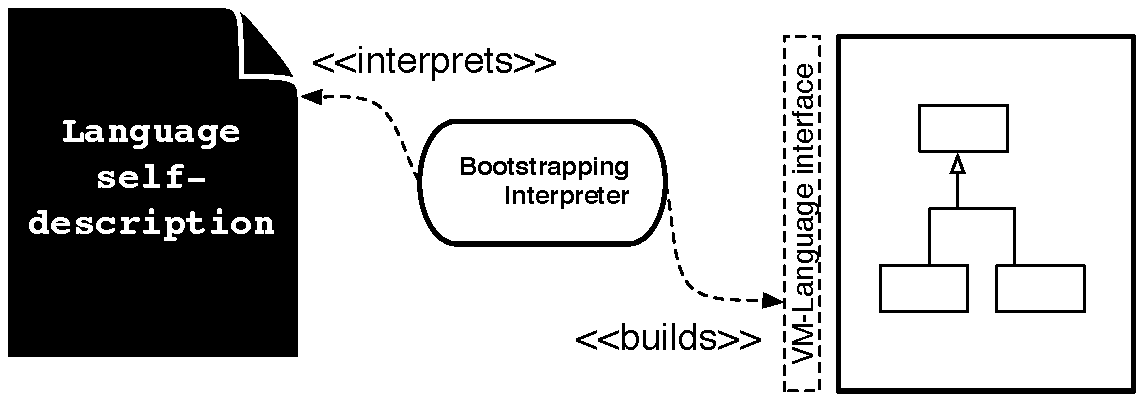
\includegraphics[width=.9\linewidth]{bootstrap_nutshell}
\caption{\textbf{Solution overview.} A bootstrapping interpreter uses the self-description in the language definition to build the language through the a clear \VM-language interface.\label{fig:bootstrapping_overview}}
\end{figure}

The main limitation of our approach is the \VM execution model. Our solution exposes a clear but fixed \VM interface that introduces a common denominator for each of the languages we bootstrapped. The co-evolution of language kernel and \VM will be addressed in future work and is out of the scope of this paper.

%============================================================================
\subsection{A Bootstrapping Process for Reflective Languages}

Bootstrapping requires a language kernel to be self-described. That is, there should exist a definition of the language expressed in the language it defines. This language definition includes the \textbf{base-level} entities of the language~(its classes and methods), and the \textbf{meta-level} entities with the means to define itself from scratch~(\eg a compiler or compiler interface to create methods and classes). The latter includes in addition the code of the bootstrapping process \ie the steps that must be followed to create a coherent and well formed language kernel~(Figure \ref{fig:language_definition}).

\begin{figure}[ht]
\center
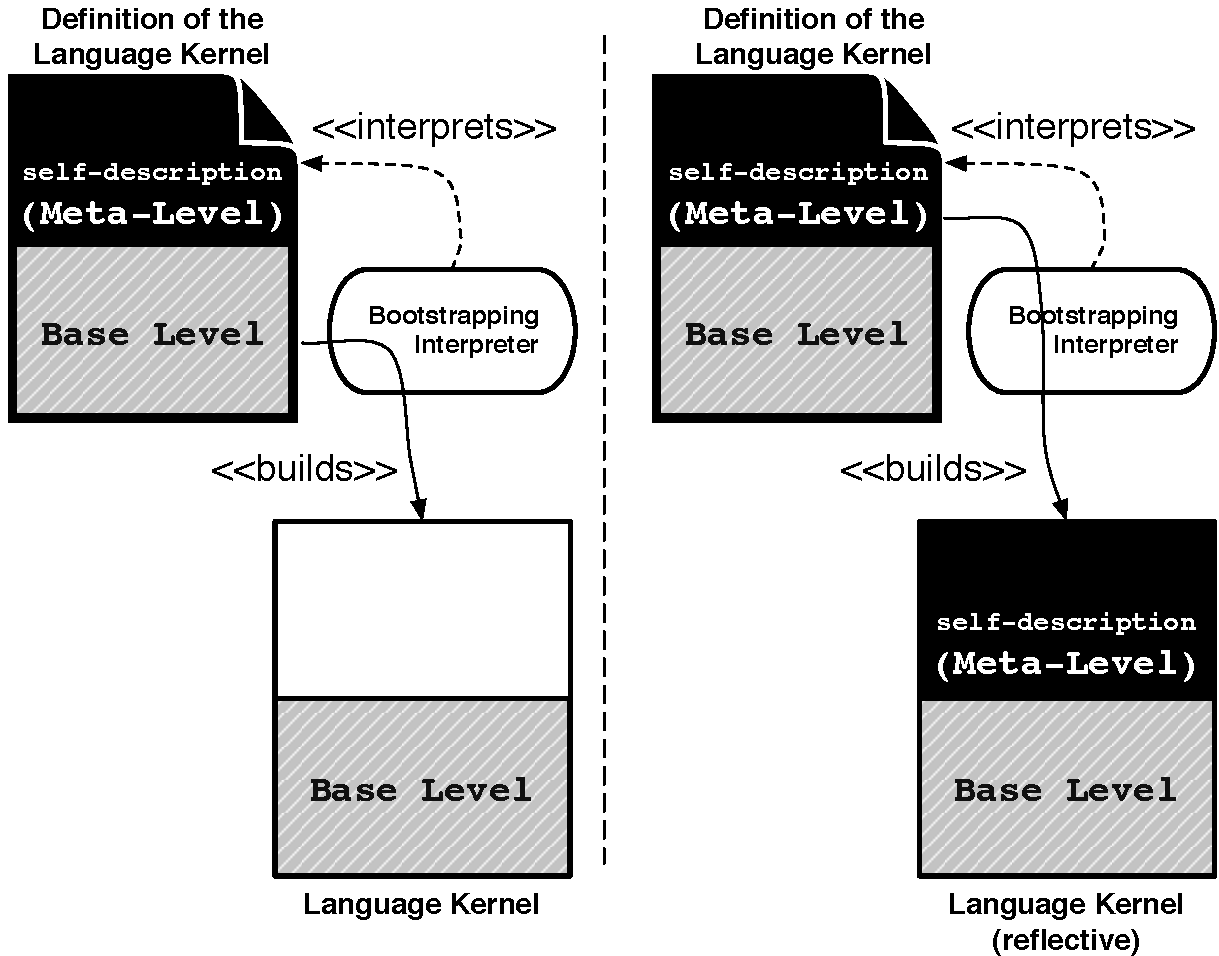
\includegraphics[width=.8\linewidth]{building_reflective_language}
\caption{\textbf{The language definition in the bootstrap process.} The bootstrapping interpreter uses the meta-level of the language to build the base-level of the language~(left-side). Afterwards, it may inject the meta-level to make it a reflective language~(right-side).\label{fig:language_definition}}
\end{figure}

Notice that although we use the language meta-level for bootstrapping purposes, it may just be needed at bootstrapping time and not at runtime. Bootstrapping does not require to inject the self-representation of the language into the language kernel. We consider that as a special case: a language kernel that includes its self-description is a \emph{reflective language kernel}.
A language that contains both introspection and full intercession facilities is a fully reflective language. A fully reflective language does not only have the minimal set of elements to run, but also the minimal to be autonomous: it can create classes and methods without any external component~(compiler, class builder, interpreter).

Thus, this language definition has direct impact on the design of the language we bootstrap. Figure \ref{fig:phases} shows the stages of a bootstrap process as it installs classes or packages inside the language kernel. When the bootstrap process starts, the language kernel is not yet able to execute code by itself \eg it cannot resolve the method lookup because the class hierarchy is not created. As we install packages or classes, we arrive at the point where the kernel contains already the minimal set of elements it needs for execution, the \emph{execution point}. Later on, we can install reflective features into the language to get inside the \emph{reflective spectrum} of languages. 

%When bootstrapping a reflective language, the language definition must ensure the causal connections that exist between the program and its representation~\cite{Maes87a}.


\begin{figure}[ht]
\center
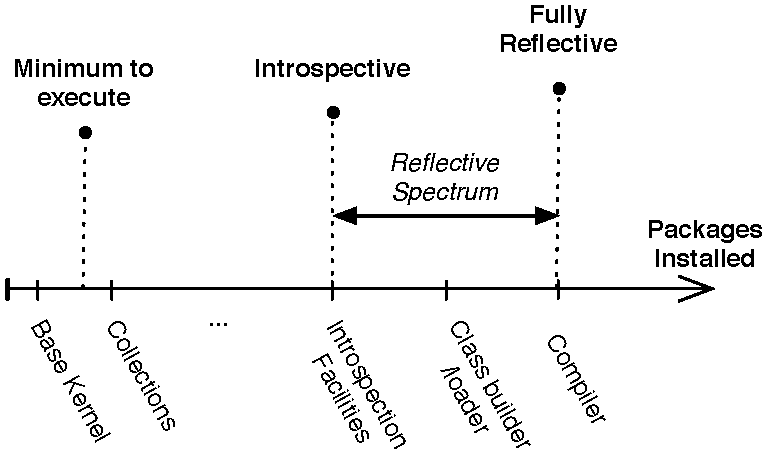
\includegraphics[width=.9\linewidth]{bootstrapping_phases}
\caption{\textbf{Bootstrap Phases.} Initially, a language kernel does not contain the minimal elements to execute code. As the bootstrap process installs elements, it reaches the point of execution where it can run autonomously. Later on, when (if) reflective features are installed, the process reaches the reflective spectrum, where a language kernel is considered reflective.\label{fig:phases}}
\end{figure}

%\begin{description}
%\item[The base-level language elements.]  We consider here those elements that are part of the \textbf{base-level}~(\eg basic language classes and libraries) of the language and also the ones in the \textbf{meta-level}~(\eg the reifications of the language runtime, a compiler interface, the class builder).
%
%\item[The meta-level language elements.]

\subsection{The process to create the language kernel}
The bootstrapping process requires a particular order as it sets up very interrelated dependencies~(sometimes meta-circular in the case of reflective languages~\cite{Stra14a,Chib96a,Maes87a,Smit84a}) amongst the language elements. The order and specifics to build the language must be described in the language definition so the bootstrapping interpreter can make use of it to orchestrate the process. This process presents also which are the elements that will be introduced into the built language: it is here where we decide if the output language kernel will be reflective or not.

Following we describe a bootstrap process we developed to bootstrap the Pharo language. A bootstrap process may be different for different languages, as they may contain different meta-models and concepts. As an example, Figure \ref{code:process} shows an excerpt of our particular bootstrap process applied to the Pharo language.

\begin{figure}[ht]
\begin{code}
Bootstrap >> bootstrap [
    "Create the basic language structures"
    nilObject := UndefinedObject basicNew.
    trueObject := True basicNew.
    falseObject := False basicNew.
    
    globalTable := GlobalTable basicNew.
    globalTable at: #GlobalTable put: smalltalk.
    
    SymbolTable initialize.
    
    "Solve the class creation bootstrapping issue"
    Class
        instVarAt: 4
        put: (FixedClassLayout
            withInstVars: #(superclass methodDict format layout ...)).
    
    "Create classes"
    ClassBuilder new
        superclass: nilObject
        subclass: #ProtoObject
        instanceVariableNames: ''.
    ClassBuilder new
        superclass: ProtoObject
        subclass: #Object
        instanceVariableNames: ''.
    ...
]
\end{code}
\caption{\textbf{Code (excerpt) of the Pharo language definition.}\label{code:process}}
\end{figure}

%In \cite{Poli13b} Polito et at. 
%we provided a detailed process to bootstrap an object-oriented reflective language such as Pharo. The bootstrap process is not the contribution of this paper. However, for the sake of completion and to aid the understanding of the rest of the paper, we briefly explain in this section the bootstrap process by the means of an example consisting in the bootstrap of the Pharo language. \gp{send them to read our report with the full blown process}


%\paragraph{Step 1: Generate the guest language AST definitions.}
%
%The builder takes as input the specification of the guest language, parses them and generates abstract syntax trees~(ASTs) of the new language's elements~(\eg classes and methods). 
%These AST objects provide to the bootstrap process with (a) the format and shape of classes and objects, (b) the source code of methods to be compiled inside the object space and used by the AST interpreter and (c) compile-time information such as instance and class variable names.

\paragraph{\textbf{Step 1: Create the first well-known objects}}\label{sec:create_nil}

When the bootstrap process starts, the bootstrapped language kernel is empty \ie there are no objects inside it. 
The first step of the process is to create the \ct{nil}, \ct{true} and \ct{false} objects needed for execution. It is important to create the \ct{nil} object first as the rest of the objects will have their fields initialized to it. \ct{true} and \ct{false} are required for code execution.
%%that are created inside the object space 
%will initially have their fields pointing to the \ct{nil} object from the guest language kernel. Then, the first object that the bootstrap process creates is the \ct{nil} object.
%
%In a class based object-oriented language\footnote{These same problems appear in the case of prototype based languages}, the expected way to create the \ct{nil} instance would be to instantiate it from its class. However, the \ct{nil} class does not exist yet in the guest language kernel. Creating it poses some recursive questions: (a) if the a class is an object, how could we create a class without another class for it? and (b) if that class must be initialized with references to \ct{nil}, how can we reference the correct \ct{nil} object if there is no \ct{nil} instance yet? To solve this issue, a \ct{nil} object is created in the guest kernel without linking it to a class, using an unsafe operation and breaking the language's invariants temporarily.

%An \emph{unsafe} \ct{createAnonymousObject} operation to create an object with no class. This operation takes as input the format describing the object to be created, creates the corresponding object, and outputs a mirror on that object. In our particular implementation, this operation introduces a temporary anonymous class in the guest and creates an object from it. This temporary class keeps some references to the \ct{nil} object from the host, breaking temporarily the isolation property. Using this operation, the guest \ct{nil} object is created. Later on, when the corresponding class of \ct{nil} is created, its class relationship is replaced, the temporary class is discarded (unreferenced and garbage collected), and the isolation is restored~(cf. Section \ref{sec:well_known}). The method responsible of the creation of the \ct{nil} object is shown in Figure \ref{code:nil_creation}. Figure \ref{fig:nil_creation} depicts the state of the guest language after this step.



%\begin{figure}[ht]
%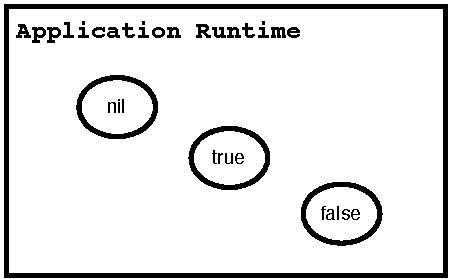
\includegraphics[width=.98\linewidth]{nil_creation}
%\caption{\textbf{State of the guest language after the creation of the classless nil object.} The \ct{nil} object is the only instance in the guest language. It is an object whose class is an anonymous class, marked in gray, pointing to the \ct{nil} object from the host.\label{fig:nil_creation} \cam{I would expect the anonymous class to appear outside the guest system rather than inside}}
%\end{figure}


\paragraph{\textbf{Step 2: Create basic language structures}}

The basic language structures of a language kernel is the minimal structure needed to create all the rest of the elements in the language. For example, the language may have a table of globally accessible objects, and a table of unique strings or symbols. These basic structures should be created from the very beginning, as the rest of the process can rely on them.
%
%
%To explain it by example, we take the well-know example of Smalltalk~(Figure \ref{fig:pharo_metaclass_metacircularity}). In Smalltalk each class has a metaclass, instance of a \ct{Metaclass} class. The \ct{Metaclass} class is an instance of a \ct{Metaclass} metaclass. According to this model, the \ct{Metaclass} class and \ct{Metaclass} metaclass should be created before any other class, and thus, it is for us the \emph{basic metacircularity}. It is worth saying that languages such as Pharo or Ruby~\cite{Mats01a} present similar models. \gp{In JavaScript... ?}
%
%\begin{figure}[ht]
%\begin{center}
%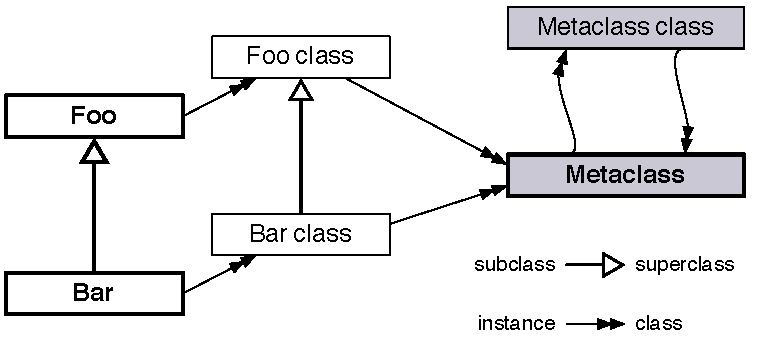
\includegraphics[width=.8\linewidth]{pharo_metaclass_circularity}
%\caption{\textbf{Metaclass metacircularity in Pharo.}\label{fig:pharo_metaclass_metacircularity}}
%\end{center}
%\end{figure}
%
%The creation of the first \ct{Metaclass} class and \ct{Metaclass} metaclass is mutually dependent: each one is an instance of the other, and thus, each one needs the other to be created. To overcome this, we use again the same strategy as for the \ct{nil} object. The builder creates the corresponding \ct{Metaclass} class and metaclass, not linking them to each other. Once both of them are available, we update their class links.

\paragraph{\textbf{Step 3: Create classes}}
We create all the classes that the language definition requires in the language kernel. The bootstrapping interpreter uses the corresponding class building mechanism in the meta-level of the language to create the corresponding classes from their descriptions. Methods are not yet installed in their classes.
%Creating a class is a complex operation at this stage. For example, a class has a name which is a symbol\footnote{a Symbol is a string unique in the system}, which in turn cannot be created yet because the Symbol class does not exist yet. Another example is the usage of complex collections such as Dictionaries in the class definitions for class variables.
%by taking each class' AST from the specification, instantiating a metaclass from the \ct{Metaclass} class and the corresponding class from the new metaclass.
% The \ct{asClassMirror} message is sent to the metaclass mirror, so the builder can instantiate the corresponding class from this metaclass. This sub step is shown in Figure~\ref{code:class_creation}. Once the bootstrap process creates all classes in this way, the guest language contains all its classes but they are still not initialized. Classes are yet not related between them and have no methods installed. Figure \ref{fig:class_creation} shows an example of the state of the guest language after this step is finished. 
%In this step the builder doesn't initialize all classes. It lets their fields referencing to the guest \ct{nil} object. No methods are installed yet.

%\begin{figure}[ht]
%\begin{code}
%newMetaclass := metaclass basicNew asClassMirror.
%newMetaclass format: aClassDefinition classSide format.
% 
%newClass := newClassMetaclass basicNew asClassMirror.
%newClass format: aClassDefinition format.
%\end{code}
%\caption{\textbf{Class creation inside the object space.} The mirror to the \emph{metaclass} allows the instantiation of a new metaclass. This new metaclass is afterwards used to instantiate the corresponding class. Each of these classes contain their corresponding formats. This task is repeated for all the classes defined in the specification. \label{code:class_creation}}
%\end{figure}
%
%\begin{figure}[ht]
%\begin{center}
%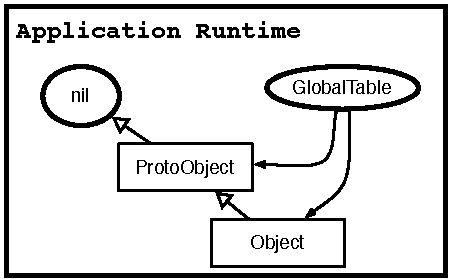
\includegraphics[width=.98\linewidth]{class_creation}
%\caption{\textbf{State of classes in the guest language after class creation.}  The metaclass metacircularity is set up. Other classes, such as \ct{Object} or the correct \ct{UndefinedObject} are instances of their respective metaclass, which in turn are  instances of \ct{Metaclass}. All slots of these classes~(in particular the slot indicating the \emph{superclass}) reference the guest \ct{nil} object. At this point, two \ct{UndefinedObject} classes exist in the guest, in gray the one created in section \ref{sec:create_nil} referencing to the host language, in white the one we created in this step. \label{fig:class_creation}}
%\end{center}
%\end{figure}

%\paragraph{Step 5: Initialize well-known instances.}\label{sec:well_known}
%
%In this step the well known instances of the language kernel are instantiated and initialized.
%We set the class link of the \ct{nil} object with its corresponding class which was created in the last step. We create also other well known instances such as the \ct{true} and \ct{false} objects.% The process uses the \ct{setClass:} operation of the mirrors to set the \ct{nil} object its corresponding class and restore the isolation of the new language. The \ct{true} and \ct{false} instances are instantiated using their corresponding classes in the object space. 
%The code executing this step is shown Figure~\ref{code:nil_fixation}. 
%After this step, \ct{nil} is not a \emph{classless} object anymore. Also, the guest language is \textbf{transitively closed}, although it is not completely initialized as shown in Figure \ref{fig:well_known_instances}.

%\begin{figure}[ht]
%\begin{code}
%theNil setClass: nilClass.
%theTrue := trueClass basicNew.
%theFalse := falseClass basicNew.
%\end{code}
%\caption{\textbf{initialising the nil, true and false instances.} Fixing the nil reference to the new nil class that was just created. The \ct{setClass:} operation of the mirrors is used. Also, the \ct{true} and \ct{false} instances are created by instantiating their corresponding classes. \label{code:nil_fixation}}
%\end{figure}

%\begin{figure}[ht]
%\begin{center}
%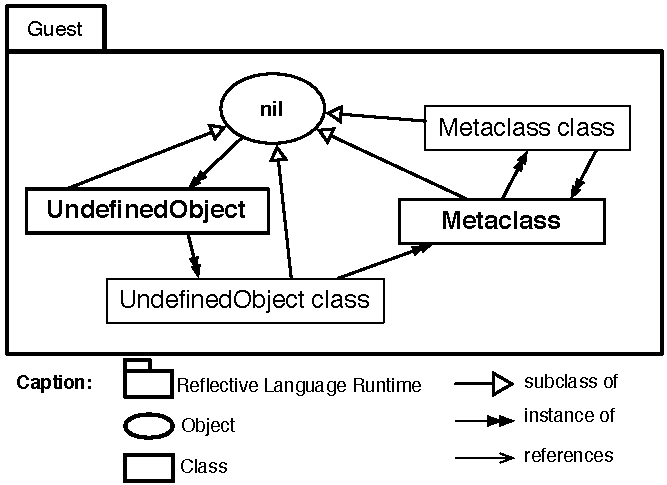
\includegraphics[width=.98\linewidth]{well_known_instances}
%\caption{\textbf{The guest language is finally transitively closed.} After setting the \ct{nil} object with its corresponding class from the guest language, the graph is transitively closed.\label{fig:well_known_instances}}
%\end{center}
%\end{figure}

%\begin{figure}[ht]
%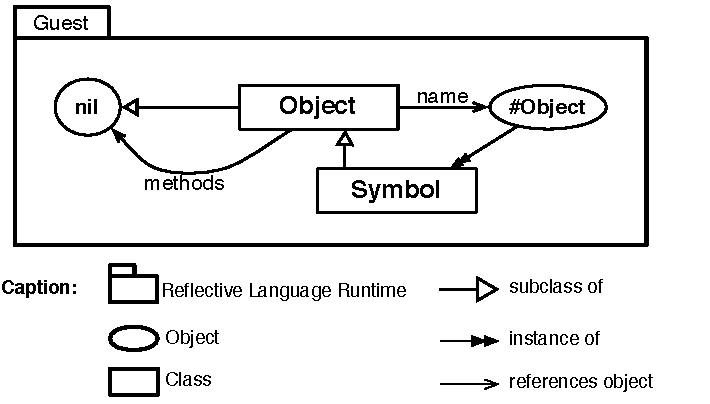
\includegraphics[width=.98\linewidth]{class_initialization}
%\caption{\textbf{State of classes in the guest language after class initialization.}  Each class references to its corresponding superclass. The superclass of \ct{Object} is \ct{nil} as it is the root of the inheritance chain. Class state is initialized~(\eg their names initialized as symbols) except their methods. \label{fig:class_initialization}}
%\end{figure}

\paragraph{\textbf{Step 4: Installing methods}}

We compile~(if needed) and install each of the methods present in the language definition into their respective classes. Method literals are bound to their corresponding literals or global objects (\eg classes).

%\begin{figure}[ht]
%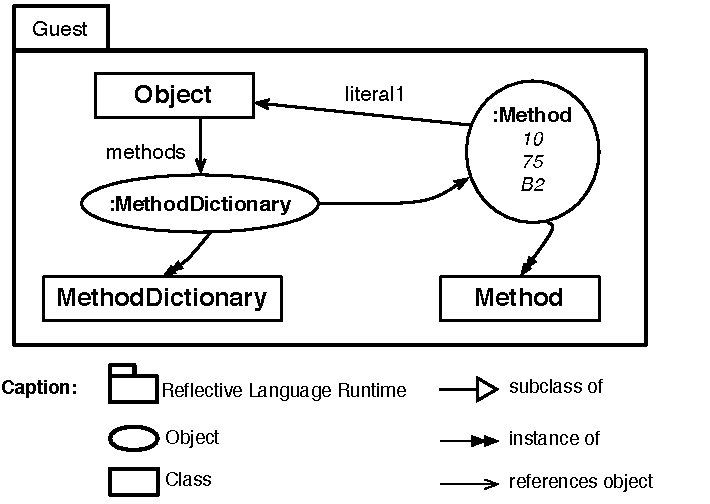
\includegraphics[width=.98\linewidth]{method_installation}
%\caption{\textbf{State of classes after method installation.} Each class has a method dictionary. Each method dictionary references the installed methods. A method object contains the bytecode and references the literals it uses.\label{fig:method_installation}}
%\end{figure}


\paragraph{\textbf{Step 5: initialization}}
%With all the classes and methods from the language specification installed, the structural part of the language is already set up. 
This last step consists in the execution of the class initialize methods to set up elements such as character tables, well-known float values~(\eg NaN or Infinity) and the thread machinery. This means that at this point, our language kernel should be able to execute code by itself.
\newline

While such a bootstrap is not difficult to express per se, it raises the question of how it can be executed. This is challenging especially, since for example we need classes to be defined to execute this exact bootstrap description. This question leads to ask ourselves about the infrastructure required to be able to manage this and other different bootstraps. The following section describes the infrastructure we built to solve this problem.

% ===========================================================================
\section{Bootstrapping with \Vtt}\label{sec:bootstrapping_infrastructure}

We implemented a bootstrapping infrastructure on \Vtt. In our solution, the bootstrapped language kernel will be created inside the virtualized runtime. This virtualized runtime is initially empty and a bootstrapping hypervisor will fill it with new objects before running the virtualized environment. The main component of the bootstrapping hypervisor is a \emph{bootstrapping interpreter}. The bootstrapping interpreter is a specialised AST interpreter that executes the code available in the language definition~(Figure \ref{fig:objectSpaceOverview}).

%  on \emph{object spaces} and abstract interpretation~(cf. Figure \ref{fig:objectSpaceOverview}). An object space is a first class representation of an \emph{object runtime system}: it is an object that provide a high level API to manipulate an object runtime system. An object space \textbf{isolates} its represented object runtime system by using mirror objects~\cite{Brac04b}~(cf. Section \ref{sec:mirrors}). Abstract Syntax Tree~(AST) interpretation solves the remaining issues. First, the combination of object spaces and the AST interpreter allow multiple object runtime systems to co-exist and execute independently, overcoming the \textbf{unicity hyphotesis}~(cf. Section \ref{section:object_spaces} and Section \ref{sec:ast_interpreter}). Second, with AST interpretation we can execute code inside the guest language kernel, using the language specification as a source for both compilation and execution, \textbf{avoiding logic duplications}.
%
%In this section, we present how our solution supports the bootstrap process introduced in Section~\ref{sec:process} and solves our stated challenges. We provide the API of both our object spaces and mirror objects, and how our AST interpreter interacts with the object space infrastructure.

\begin{figure}[ht]
\center
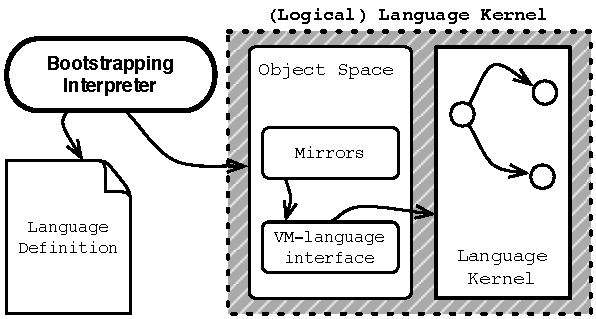
\includegraphics[width=.9\linewidth]{object_space_bootstrap_overview}
\caption{\textbf{Solution overview.} An object space provides with a clear interface to manipulate the bootstrapped language kernel. The AST interpreter interprets the language definition and uses the object space interface to manipulate the language kernel.\label{fig:objectSpaceOverview}}
\end{figure}

To support the bootstrapping process in the time, our bootstrapping infrastructure supports also the idea of continuous bootstrapping \ie integrating the bootstrapping process in a continuous integration environment where changes are common and bootstrapping must be performed continuously.

\subsection{Virtualized Runtime for Bootstrapping}\label{section:object_spaces}

We based our infrastructure on the object space model~\cite{Poli13a}. Following this model, an object space is a first-class representation of an object runtime system, meant for its manipulation and control. The object space model provides a framework to encapsulate and manipulate the runtime system where our language kernel will be bootstrapped. When bootstrapping, this object space is initially empty and the bootstrapping interpreter fills it with classes as the bootstrap process advances.

We use an object space with two main purposes: first, as a \VM interface with the bootstrapping interpreter, allowing us to bootstrap our language kernel directly inside a \VM heap; second, once the language kernel is bootstrapped we use it to initialize the \VM with it and run it. By introducing object spaces into the bootstrapping infrastructure, we clarify the interface between the language kernel and our \VM, allowing us to have different language models as long as they respect this interface. The object space model presents an \ct{objectSpace} interface that provides with general operations and mirror objects~\cite{Brac04b} with operations to manipulate individual objects. Following, we describe this interface, focusing on those operations used by the bootstrap process.

\begin{code}
objectSpace {
    /* For bootstrapping purposes when no class is available */
    mirror allocateObjectOfSize(int size);
}
\end{code}

\subsection{The Bootstrapping Interpreter}\label{sec:ast_interpreter}

The bootstrapping interpreter is a code interpreter, potentially written in language different from the bootstrapped one, that interprets code expressed in the bootstrapped language. Its design present the following important points that allow it to execute code inside the language kernel before it reaches the execution point:

\begin{description}
\item[Alternative method lookup.] Before reaching the execution point, the class hierarchy of the language kernel is incomplete, or part of its methods is not yet installed. An alternative method lookup mechanism is put in place in the bootstrapping interpreter to allow message sending before we reach the execution point: methods are looked up in the definition of the language instead of the hierarchy in the language kernel; a mapping is kept between classes created in the language kernel and their definitions in the language definition to know where the lookup should start.

\item[Automatic class stubs.] The bootstrapping interpreter does also solve most of the well known bootstrapping issues~(\eg how to create a class before a class exists) in a generic way by using class stubs. When an inexistent class is needed during the bootstrap process, the interpreter creates an empty class to take it place respecting the \VM format for it. The interpreter will be able to create instances of this class and map it to its corresponding definition to perform the method lookup. This class cannot, however, initially perform reflective operations as it does not contain any reflective information. When the real class is created later on in the process, it replaces the stub.

\end{description}

\begin{figure}[!ht]
\center
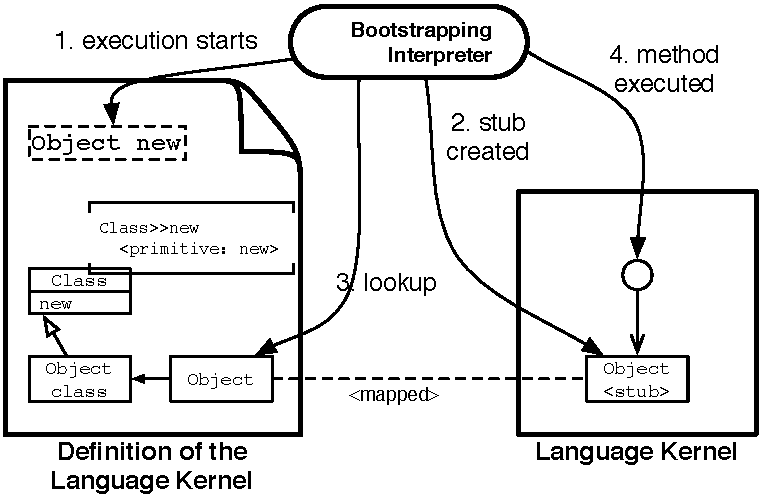
\includegraphics[width=.8\linewidth]{interpretation}
\caption{\textbf{The Bootstrapping interpreter in action.} A stub class is created for a non existent class. Each class is mapped to its description in the language definition. The lookup is then performed inside the language definition. Once the method is found, it is executed inside the language kernel.\label{fig:interpretation}}
\end{figure}

Figure \ref{fig:interpretation} illustrates with an example the behavior of the interpreter, particularly in the execution of the \ct{"Object new"} expression. First, if the class \ct{Object} does not exist, it create a stub \ct{Object} class and maps it to its corresponding definition in the language definition. To interpret the \ct{new} message, the interpreter performs the method lookup from the class of the object in the language definition. As the class from the language kernel and the language definition are mapped, the interpreter knows where to start the method lookup. Finally, the found method is executed in the language kernel and an instance of the \ct{Object} class is created.



By using the bootstrapping interpreter to bootstrap, all the executed logic comes from a single source: the language definition. This avoids  major code and logic duplications as the only one point for extension or modification of the bootstrapped language is its definition. Figure~\ref{code:logic_dup3} illustrates how we can use the interpreter to use the \ct{Dictionary} definition from the language and avoid duplications shown in Section \ref{sec:problems}.


\begin{figure}[ht]
\begin{code}
Bootstrap>>createDictionaryWith: n
    "Create a dictionary in the new language kernel"
    ^ interpreter
            execute: 'Dictionary new: size'
            binding: { 'size' -> n }.
\end{code}
\caption{\textbf{Avoiding logic duplications with the bootstrapping interpreter.} This example shows how the bootstrapping interpreter does not duplicate the logic of the \ct{Dictionary>>initialize} method, but uses it instead.\label{code:logic_dup3}}
\end{figure}


\subsection{Continuous Bootstrapping}

Building continuously a language kernel provides the language engineers with the same benefits of continuously building another application: automated integration and testing, quick and continuous feedback on the applied changes. This continuous feedback should give the language developer with the information and tools to resolve conflicts and problems: it should clearly show which was the \emph{impact} of such change in the process. A change introduced in the language impacts directly on the definition of the language~(Figure \ref{fig:impact}). The changed definition is used in turn by the bootstrap process to bootstrap the new version of the language kernel, thus the change has also an indirect impact on the bootstrapped language. 

\begin{figure}[ht]
\center
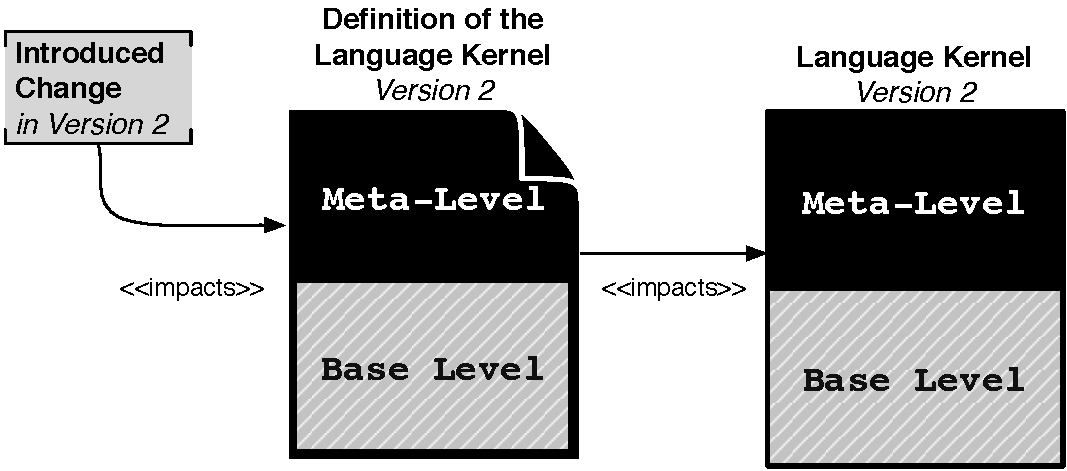
\includegraphics[width=0.7\linewidth]{impact}
\caption{\textbf{How a change impacts the bootstrap process.} A change in the language may impact directly in the definition of the language, which in turn impacts in the bootstrapped language.\label{fig:impact}}
\end{figure}

However, not every change in the language definition may impact the bootstrap process: not all the code in the language definition is used during the bootstrap~(\ie executed by the bootstrapping interpreter) and not every change impacts in the behavior of the process (\eg changing the set of final classes introduced by the bootstrap). With this purpose we introduced as a second output of our bootstrapping interpreter, an execution trace containing all the language elements that were used to bootstrap: any change on these elements may have an impact on the process. Then, to produce useful feedback for the changes made by a language developer, an \emph{impact resolver} measures the impact of a change in the bootstrap process by comparing the introduced change to the previous bootstrap execution~(Figure \ref{fig:resolving_impact}).

Our bootstrapping infrastructure measures the impact by making a diff between the traced and changed language elements. In case a change breaks the bootstrap process, the language engineer has enough information to spot the problem and act on it.

\begin{figure}[ht]
\center
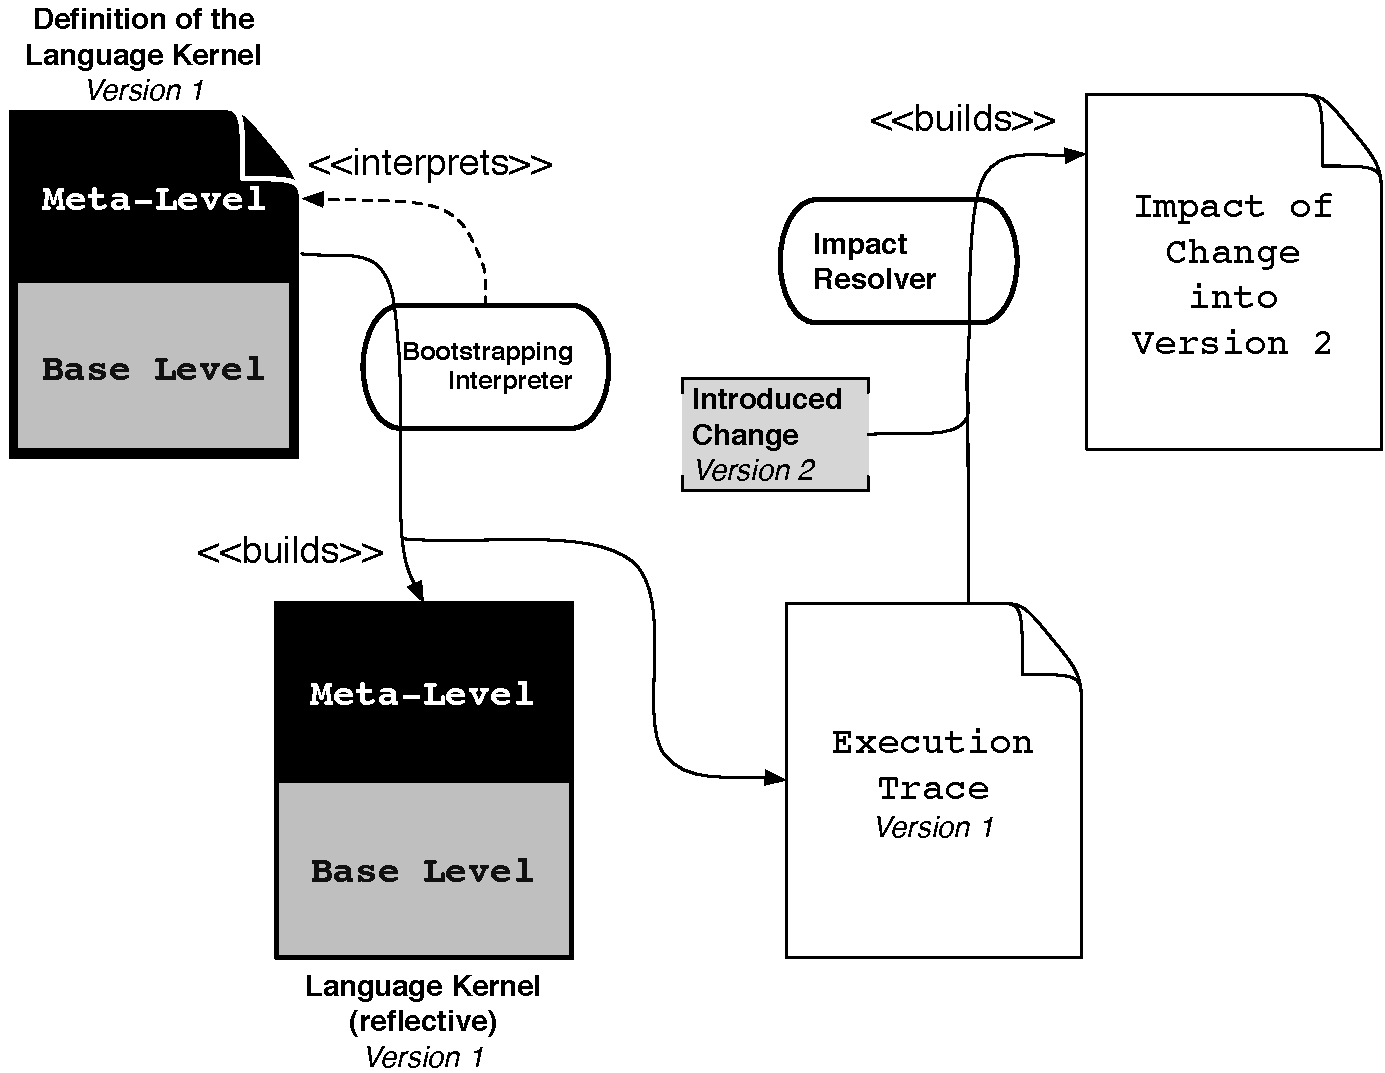
\includegraphics[width=.8\linewidth]{resolving_impact}
\caption{\textbf{How a change impacts the bootstrap process.} The bootstrap process execution is traced. An impact resolver decides if the introduced change will impact in the bootstrap process or not.\label{fig:resolving_impact}}
\end{figure}

% ===========================================================================
\section{Validation} \label{sec:bootstrapping_validation}

In this section we present our results while bootstrapping three different three different case study languages.
As all our languages share the same \VM, we start this section by describing the execution model of this \VM and its impact on the bootstrapping languages.
To reuse the parsing infrastructure and the bootstrapping interpreter, the three bootstrapped languages share also the same syntax: a Smalltalk syntax. Although these similarities, each of the three language kernels possess different model and semantics: Pharo is a fully-reflective language composed of classes and traits with first class slots and object layouts \cite{Verw11a}; \emph{Metatalk}~\cite{Papo11a} is a language that fully decomposes the meta-level from the base-level using mirrors, allowing us to bootstrap a reflective and a non-reflective version of it; \emph{Candle} is a partially reflective \ct{Smalltalk-80} based mini-kernel that includes introspection and some self-modification features. Figure \ref{fig:languages_spectrum} shows how these three languages are placed in the language spectrum.% These results show that our process can produce different systems when fed with different specifications. The resulting bootstrapped systems are available at \url{http://ci.inria.fr/rmod/view/Oz/}.

\begin{figure}[ht]
\center
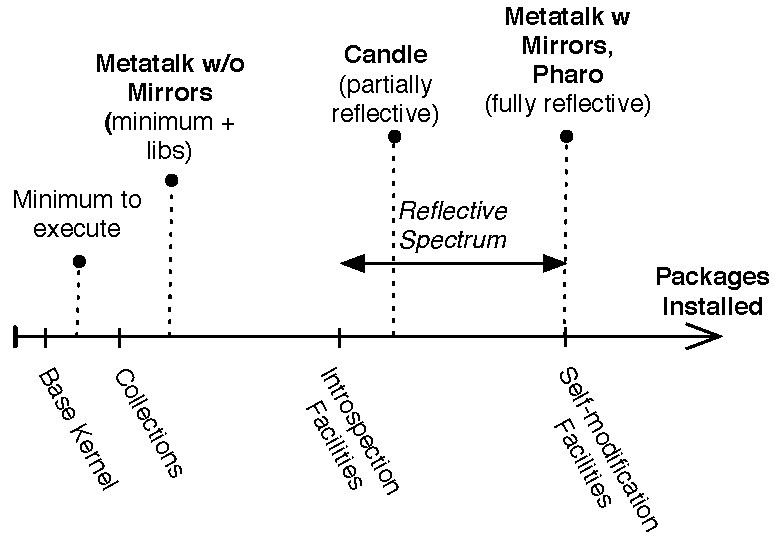
\includegraphics[width=.8\linewidth]{languages_by_reflectiveness}
\caption{\textbf{Bootstrapped Languages Spectrum.} How the languages we bootstrapped are placed in the phases and reflective spectrum. In particular, Metatalk with and without its mirrors is in different extremes of the spectrum.\label{fig:languages_spectrum}}
\end{figure}

Finally in this section we present some measurements. To keep bootstrapping practical, we optimized the critical parts of the process for both the language user and the language engineer. On one side language users do not usually search to modify the language kernel but to use it, independently of the language initialization process it provides. To suit this scenario we do not build the language kernel each time: we generate a snapshot with a cached version of it. On the other side we find language designers/engineers whose job is to change the language kernel. For them the bootstrap process must provide with an acceptable development cycle for activities like debugging. With this case in mind, we optimized the \emph{bootstrapping interpreter} with a dynamic compilation technique. Each of the measurements we present below were made on a 2.2 Ghz Intel Core i7 machine with memory 8 Gb 1333 Mhz DDR3.


\subsection{Pharo Execution Model in a Nutshell}\label{sec:pharo_execution_model}

To understand the common denominator between the three language kernels we bootstrapped, we describe briefly the execution model imposed by the Pharo \VM. The Pharo \VM features a bytecode-based stack interpreter with a generational garbage collector and a JIT compiler. For the interested reader, several publications describe its details and how it evolved during time~\cite{Gold83a,Inga97a,Mira11a}. On the execution model side, this \VM imposes us the following contract:

\begin{description}

\item[Object Format.] All objects in a Pharo \VM have a header and a list of fields. The object header is one, two or three words long and describes amongst others how large is the field list of the object, if those fields contain weak or strong pointers, and which is the class of the object.

\item[Object Model.] The Pharo \VM enforces, in its lowest level, a class-based object oriented model with single inheritance. Each object has a reference to its class~(that appears inside its header). Additionally, each class has three mandatory fields: the class format is used to create new instances and the class' superclass and a method dictionary are used during the method lookup. The \VM during its execution does not enforce the existence of metaclasses nor a particular class hierarchy. This simple model allows one to implement language extensions such as Traits~\cite{Scha03a}.

\item[Bytecode set.] The Pharo \VM constrains methods to a single bytecode set, based on its stack machine. This means that every language that is meant to run on top of this \VM must be compiled to this bytecode set, independently of its original syntax and semantics. 

\end{description}

\subsection{Case Study I: Pharo}\label{sec:bootstrap_pharo}

Pharo~\cite{Blac09a} is an object-oriented reflective Smalltalk-inspired programming language. As it is a Smalltalk-80 inspired language, its class model includes implicit metaclasses: each class has its own metaclass, an instance of \ct{Metaclass}. Pharo also extends the execution model its \VM provides with traits~\cite{Scha03a} and class extensions~(\ie the ability to add methods to a class that belongs to another package). Finally Pharo has first class instance variables (slots) structured in object layouts \cite{Verw11a}. Figure \ref{fig:pharo_simplified_model} shows how the elements of the language are related to each other; the diagram is not meant to reflect the actual class graph but the language concepts.

\begin{figure}[ht]
\center
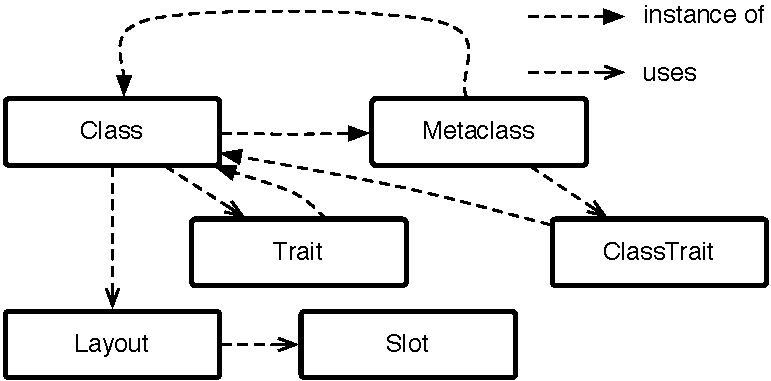
\includegraphics[width=.7\linewidth]{pharo_simplified_model}
\caption{\textbf{Simplified Pharo object model schema.} In Pharo each class has a metaclass. Metaclasses are defined circularly. Both classes and metaclasses makes use of trait objects to define part of their behavior. Classes also has layout that organises first class instance variables (slots). This schema does not represent the actual object graph, but a simplified picture.\label{fig:pharo_simplified_model}}
\end{figure}

Pharo is a fully-reflective language, placed at the end of the reflective spectrum. The Pharo language includes introspection in the kernel itself, and also self-modification stratified in three levels: object mutation facilities, a class builder and a compiler. The main challenge in Pharo is that the kernel itself of Pharo is defined by Traits: \eg the Trait class uses a Trait. First class slots also add to the self-description of the language. This introduces new bootstrapping issues that must be resolved at bootstrapping time.

%Our resulting language kernel includes the packages defining Pharo's class model, traits, collections, the process scheduling library, the compiler and the class builder. The two latter allow the system to be extensible without external tools. With this selection we bootstrapped a language kernel that represents the 19\% of the original language kernel.
%The memory  the resulting bui language is 2MB, contrasting its 22MB original counterpart. \gp{remeasure it. Do we care about size?}

%Regarding its health, the boostrapped kernel can be tested using the SUnit testing framework.
%Unit tests of the kernel itself are loaded using the binary loader and run in the new system.
%Using this same mechanism, core packages like the compiler are able to be tested isolated from other libraries.

%A peculiarity of this system is that it is capable of bootstrapping a copy of itself.
%This is achieved by loading the binary packages of hazelnut and using it's own specification in the building process.
%Regarding the size of our obtained kernel, which is certainly not yet the minimal possible, our results shows that the design of the language kernel should be refined to create an even cleaner version.

\subsection{Case Study II: Metatalk} \label{sec:bootstrap_metatalk}

Metatalk~\cite{Papo11a} is a reflective language where reflection is fully decomposed in explicit meta-objects, namely mirrors~\cite{Brac04b}. Metatalk makes the usage of reflection explicit: a program's execution takes place in the base-level of the language kernel, and it jumps to a meta-level when a mirror is used. Metatalk class model is simpler than Smalltalk's class model. It does not impose metaclasses. Instead, all classes are instances of the single \ct{Class} class. If there is a need for metaclasses~(to share behavior between classes), the developer can write its own explicit metaclasses~(Figure \ref{fig:metatalk_simplified_model}).

Metatalk mirrors decompose reflective behavior as well as the language meta-information \ie class' names, field order and names amongst others are part of its mirrors, and thus, they belong to the meta-level. When there is not a need for reflection, a Metatalk program can discard its meta-level with all the meta-information in it. This decomposition allows us to bootstrap Metatalk with or without its meta-level. This results in two different language kernels: Metatalk base-level has no reflection at all, while Metatalk with both the base and the meta level is a fully-reflective language.

\begin{figure}[ht]
\center
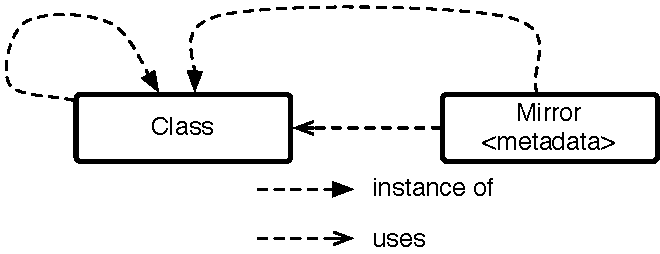
\includegraphics[width=.7\linewidth]{metatalk_simplified_model}
\caption{\textbf{Simplified Metatalk object model schema.} In Metatalk classes have no implicit metaclass. All classes share the same class. Mirrors are simple objects, thus instances of classes, that reflect on a class and contain their metadata. This schema does not represent the actual object graph, but a simplified picture.\label{fig:metatalk_simplified_model}}
\end{figure}

Metatalk's can be bootstrapped in two different ways. A non-reflective bootstrap initializes only the main classes of the language but does not create its meta-level. The non-reflective bootstrap does not contain mirrors. A second bootstrap creates a reflective Metatalk, which based on the latter one introduces the mirror instances with their corresponding metadata. We could bootstrap easily Metatalk in such a way due to the clear decomposition of its reflective elements. 

%%%%%%%%%%%%%%%%%%% Case of study and Results 2 %%%%%%%%%%%%%%%%%%%%
\subsection{Case Study III: Candle} \label{sec:bootstrap_candle}

Candle is a Smalltalk-based language with a micro language kernel. Its class model includes implicit metaclasses as Smalltalk's and Pharo's one. However, Candle has no support for traits or slots~(Figure \ref{fig:candle_simplified_model}). We built Candle's language kernel by adapting MicroSqueak~\cite{Malo11a} to run on top of the Pharo \VM. This micro language kernel was designed with the explicit goal of being the minimal distribution for the Squeak Smalltalk language.

\begin{figure}[ht]
\center
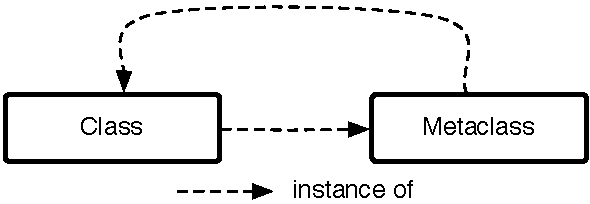
\includegraphics[width=.6\linewidth]{candle_simplified_model}
\caption{\textbf{Simplified Candle object model schema.} Candle follows a more traditional Smalltalk-80 model. In Candle each class has a metaclass. Metaclasses are defined circularly. There are no traits. This schema does not represent the actual object graph, but a simplified picture.\label{fig:candle_simplified_model}}
\end{figure}


Candle is a partially reflective language defined by a total of 49 classes and a reduced set of methods. Candle includes a minimal core of the language, a basic collection library and basic file IO support. It also provides with object introspection and mutation facilities. It does not include, however, a class builder or compiler to extend itself.%A bootstrapped Candle kernel presents a memory footprint of 80KB, with potential applications in embedded devices with little available memory.\gp{remeasure it. Do we care about size?}

\subsection{Measurements}

In this section we present the benchmarks we did to measure the bootstrap time of each of our three languages using our standard infrastructure. Table \ref{tb:measurements} shows the time to bootstrap each of the three languages using an unoptimised AST interpreter. This time comprehends the entire bootstrap process: from parsing the code in the language definition to its complete setup. We executed each of these benchmarks 10 times. The results table puts also the results in context: it presents how many code entities~(classes, traits, mirrors) and methods are built for each language. Notice that the bootstrapping time depends on the amount of elements it builds and also on their complexity. For example, creating a class in Pharo involves a biggest graph of objects than in the other two languages (because of the introduction of traits and class layouts). Section \ref{sec:optimisations} introduces two optimizations we did based on these measurements, that focus on the startup time and the development cycle of the bootstrap. 

 \begin{table}[ht]
 \small
 	\centering
 	\begin{tabular}{|l|c|c|}
			\hline
			\textbf{Language}
			& \xspace\textbf{Code entities / Methods}\xspace
			& \xspace\textbf{Bootstrap time}\\
		\hline
		Pharo & 626* / 6812 & 9004756ms +/-621265 \\\hline
		Candle & 100* / 875 & 86747ms +/-8060 \\\hline
		Metatalk w/o mirrors & 25 / 114 & 957ms +/-112 \\\hline
		Metatalk reflective & 58* / 166 & 13697ms +/-61 \\\hline
 	\end{tabular}
		\vspace*{0.2cm}
 	\caption{\small\textbf{Building Benchmarks.} Comparing the execution time of the bootstrapped languages using AST interpretation and partial evaluation. (*) Pharo and Candle have implicit metaclasses, meaning that for each created class, an associated metaclass is created even if not necessary. Metatalk introduces a mirror object for each of the classes in the language.\label{tb:measurements}}
 \end{table}

We can observe from our measurements that bootstrapping Metatalk takes in average 1 second if no mirrors are created and 13 in the reflective Metatalk case. Candle bootstrap is slower, in the order of 1 minute and a half, mainly because it contains eight times more methods than the Metatalk. We can see that a plain AST-based bootstrapping interpreter has a a bigger impact in the bootstrap time if the language contains complex structures to initialize.  Indeed, creating a Pharo class using the AST interpreter is an operation that takes in average 17 seconds, because each class contains a reification of its memory layout and slots~\cite{Verw11a}. This problem is aggravated by the high amount of classes and methods in this language definition.

Particularly about bootstrapping Pharo, a lack of modularity of the language impacts in the amount of code elements we have to build. Pharo's language kernel is historically a monolithic system which precludes us to build a minimal system. In fact, the Pharo language kernel we are bootstrapping represents a subset of the full Pharo language as it is distributed.

\subsection{Optimisations}\label{sec:optimisations}

To be useful in practice, we understand that the bootstrap process should have the following two properties: (a) be fast enough to provide a good feedback loop and allow debugging to the language engineer and (b) provide a short startup time for the language users. Optimising a bootstrap process is indeed a challenge since we cannot optimise it statically by fixing the meta-level semantics, as changing them is the main purpose of the bootstrap. In the following sections we show how snapshotting and dynamic compilation aid in these two optimisation scenarios. 

\begin{description}
\item[Enhancing Bootstrap Time: Dynamic Compilation.]
Since the main purpose of the bootstrap process is to easily change the meta-level semantics and structure of the language entities we cannot fix them statically to optimize them. In exchange, we chose to optimize the interpretation cycle using a dynamic compiler. The dynamic compiler compiles the interpreted code on demand. This compiled code is cached and executed directly on the \VM bypassing the interpretation step in following executions. We implemented dynamic compilation to optimize Pharo as it presents the worse of our results~(cf. Table \ref{tb:dynamic_compilation}). We reduced the total bootstrap time by a factor of 2.85. Additionally, we observed a mayor improvement on class creation, where the time improves from 17 to less than half a second. Class creation has a great impact on the Pharo's total bootstrap time, as it is executed 313 times. Contrastingly, the initial setup of the language structures~(\eg the symbol and character table, the initial threads) is executed only once where the cost of our dynamic compilation implementation increases the execution time. Please notice that the current implementation does not optimize method compilation nor parsing, meaning there is still a room for improvement.

 \begin{table}[ht]
 \small
 	\centering
 	\begin{tabular}{|l|c|c|c|}
			\hline
			\textbf{Case}
 			& \textbf{AST Interpretation}
			& \textbf{Dynamic Compilation}
			& \textbf{Gain Factor}\\
		\hline
		Total Bootstrap & 9004756ms +/-621265 & 3158525ms +/-219334 & 2.85x\\\hline
 		Initial Setup (Symbol table, etc.) & 247621ms +/-9875 & 319630ms +/-40333 & 0.77x\\\hline
		Creation of one class & 17216ms +/-1401 & 432ms +/-189 & 39.85x\\\hline
 	\end{tabular}
	\vspace*{0.2cm}
 	\caption{\small\textbf{Comparison of bootstrap time in absence and presence of dynamic compilation.}\label{tb:dynamic_compilation}}
 \end{table}

\item[Optimising Startup Time: Snapshotting.]\label{sec:snapshot}
The user of a programming language is concerned about writing applications that run on this programming language instead of changing the programming language. From a user perspective the initialization of the language is transparent within the startup of an application. It should be however fast and ensure always the same state.
The language initialization present in state of the art \VMs~(Section \ref{sec:intro}) provides both properties. Bootstrapping, in the sense of this paper, turns this process slower due to the interpretation step.

For language users, we overcome this slow-down by \emph{caching} the result of our bootstrap process in a snapshot. Thus, we bootstrap a language kernel only when we change it, and otherwise we load the cached version. Caching keeps both properties of application startup: it guarantees the same state and it is faster. Table \ref{tb:startup} shows a comparison in the startup time of our \VM loading Pharo and Candle using snapshots, in contrast with Ruby. We measured the startup times by running each of them 10 times and making an average. From the results, we observe our startup time is bigger than ruby's but still reasonable, under the half of a second.

 \begin{table}[ht]
 \small
 	\centering
 	\begin{tabular}{|l|c|}
			\hline
			\textbf{Language}
 			& \textbf{Startup time}\\
		\hline
		Ruby &  64ms +/-7.1\\\hline
		Pharo & 280.8ms +/-3.4\\\hline
		Candle & 186ms +/-7.6\\\hline
		Metatalk w/o mirrors &202ms +/-13\\\hline
		Metatalk reflective &205ms +/-11\\\hline
 	\end{tabular}
	\vspace*{0.2cm}
 	\caption{\small\textbf{Startup time in perspective.} Comparing the startup time of a ruby application with the same in Pharo or Candle using a snapshot.\label{tb:startup}}
 \end{table}

Implementation-wise, the snapshot we used is a memory dump of the \VM heap. This heap will contain all the objects, classes and methods we created during the bootstrap. At load time, the memory dump is restored into memory and the \VM internals are re-configured to use this heap using the \VM setup interface~(Section \ref{section:object_spaces}). This idea is the same used by languages such as Smalltalk, Lisp, Javascript in V8 or the JikesRVM~\cite{Alpe00a}. Loading a binary image is as fast as reading the file and putting its contents inside the \VM's heap.

\end{description}

% ===========================================================================
\section{Conclusion and Summary}

% =============================================================================
\input{chapter-footer.tex}